\documentclass[11pt]{article}
\usepackage[margin=1in]{geometry}
\usepackage{booktabs}
\usepackage{longtable}
\usepackage{array}
\usepackage{graphicx}
\usepackage[hidelinks]{hyperref}
\makeatletter
\setlength{\@fptop}{0pt}
\makeatother
\title{Supplementary Information: Extreme heat exposure around documented high-rise building fires worldwide}
\author{Author names to be confirmed}
\date{}
\renewcommand{\figurename}{Supplementary Figure}
\renewcommand{\tablename}{Supplementary Table}
\begin{document}
\maketitle
\section*{Supplementary Note 1: Evidence population and estimand}
The underlying population is the set of high-rise building fire events that could be identified and documented from the searched public sources, not all high-rise fires worldwide. The primary occurrence estimand is the within-location odds ratio comparing locally extreme-hot event days with matched non-event days in the same month and weekday. It is identifiable without a global fire-reporting denominator only if, within each short matched stratum, documentation is not itself caused by day-to-day weather after conditioning on the event. Cross-country or annual raw record counts do not satisfy that condition and are therefore descriptive.

\section*{Supplementary Note 2: Cohort construction}
\begin{longtable}{>{\raggedright\arraybackslash}p{0.2\textwidth}>{\raggedright\arraybackslash}p{0.16\textwidth}>{\raggedright\arraybackslash}p{0.55\textwidth}}
\caption{\textbf{Analytical cohorts and operational definitions.}}\label{tab:s1}\\
\toprule
Cohort & Size & Operational definition\\
\midrule
All records & 239 & Every row in the updated workbook; no event deletion.\\
Valid geocode & 233 & Latitude in $[-90,90]$ and longitude in $[-180,180]$.\\
Extended & 228 & Valid date and geocode; excludes aviation, warfare, missile and comparable external triggers.\\
Core & 191 & Extended cohort with traceable official, institutional or news source and no exact duplicate candidate.\\
\bottomrule
\end{longtable}

\section*{Supplementary Note 3: Exposure specification}
The 1991--2020 ERA5-Land baseline is fixed before outcome analysis. The primary threshold is $\max(P_{90,local},30\,^{\circ}\mathrm{C})$. A day is exposed if daily maximum temperature exceeds this threshold on that day and the two preceding days. The GEE table also retains the current day and three lags together with local P85, P90 and P95 values, so every implemented threshold and duration sensitivity is reconstructed from the same ordered daily series rather than from separate post-hoc downloads. NASA POWER sensitivity data are processed by the identical baseline, threshold and lag algorithm in a separate table; they are never combined with ERA5-Land values. The descriptive seven-day score is
\[
S=\min\left(100,10\sum_{d=-6}^{0}\max\left[T_{\max,d}-\max(P_{90,local},30),0\right]\right).
\]
This bounded score was designed only for consistent map symbology. Its truncation improves visual comparability but discards variation above 10 cumulative degree-days; inferential models therefore use the binary sequence indicator and untruncated temperature anomaly.

\section*{Supplementary Note 4: Prespecified sensitivity analyses}
\begin{longtable}{>{\raggedright\arraybackslash}p{0.22\textwidth}>{\raggedright\arraybackslash}p{0.32\textwidth}>{\raggedright\arraybackslash}p{0.37\textwidth}}
\caption{\textbf{Prespecified and planned sensitivity analyses.}}\label{tab:s2}\\
\toprule
Dimension & Alternative & Purpose\\
\midrule
Heat threshold & P85, P90 and P95 with the 30\,$^\circ$C floor & Test dependence on relative-extreme definition.\\
Duration & 2, 3 and 4 consecutive days at P90 & Test temporal persistence assumption.\\
Absolute floor & 30\,$^\circ$C versus no floor & Separate absolute thermal load from local anomaly.\\
Climatology & Calendar month; a 15-day calendar window is future sensitivity work & Prevent an unimplemented alternative from being presented as completed.\\
Lag & Current day, three ordered lags and their four-day mean fitted as continuous anomalies & Test acute timing without selecting a post-hoc best curve; report Holm-adjusted values.\\
Sources & Core versus extended versus all geocoded & Assess dependence on provenance criteria.\\
Period & Exclude 2025--2026 & Assess active database-expansion period.\\
Event type & Exclude construction, façade or arson events in turn & Assess heterogeneous ignition pathways.\\
Geography & Leave-one-continent-out & Identify whether one region drives the estimate.\\
Weather product & NASA POWER MERRA-2/GEOS-IT & Test sensitivity to an independent, coarser reanalysis and processing stream.\\
\bottomrule
\end{longtable}

\section*{Supplementary Note 5: External data provenance}
ERA5-Land weather is resolved at approximately 9--11 km and should not be described as building-scale temperature. All 995 matched dates in 228 strata completed in Earth Engine. Values were sampled at the event-coordinate ERA5-Land pixel; where the land mask returned no value at a coastal point, all dates in that stratum used a documented 20-km spatial mean. Five strata required this fallback and were excluded together in sensitivity analysis. NASA POWER Release 10 meteorology is coarser, at 0.5\,$^\circ$ latitude by 0.625\,$^\circ$ longitude, and the Daily API defaults to local solar time. Its MERRA-2 stream is followed by near-real-time GEOS-IT values; 68 matched-day rows within two months of access are therefore flagged as provisional. All 1,004 matched dates returned a completed request status, 1,001 contained the complete covariate set, and the request manifest contains all 159 unique coordinates. GPW population count is used at its native 30 arc-second grid, yielding an approximately 1-km cell whose surface area varies slightly with latitude. GHSL 100-m pixels are aggregated to an approximately 1-km$^2$ neighbourhood; these represent mapped built surface, volume and average height, not the attributes of the incident building. World Bank indicators are country-year context variables with at most three years of backward matching and no forward imputation. Taiwan events remain without WDI matches.

\begin{longtable}{>{\raggedright\arraybackslash}p{0.18\textwidth}>{\raggedright\arraybackslash}p{0.19\textwidth}>{\raggedright\arraybackslash}p{0.22\textwidth}>{\raggedright\arraybackslash}p{0.305\textwidth}}
\caption{\textbf{External and author-compiled data sources.}}\label{tab:s3}\\
\toprule
Dataset & Support & Analytical role & Identifier and access boundary\\
\midrule
Author-compiled events & Point/date, 2000--2026 & Event outcome and reported consequence & Input SHA-256 recorded; source-specific redistribution review required.\\
ERA5-Land Daily Aggregated & Daily, approximately 11.1 km & Maximum temperature, dewpoint, precipitation and wind & \texttt{ECMWF/ERA5\_LAND/}\newline\texttt{DAILY\_AGGR}; Copernicus acknowledgement required.\\
NASA POWER Release 10 & Daily local solar time, 0.5\,$^\circ$ by 0.625\,$^\circ$ & Independent MERRA-2/GEOS-IT weather-product sensitivity & POWER Daily API v2.9.7; service version, source stream, request URL and access time retained.\\
GPWv4.11 & 2020, 30 arc-seconds & Native-cell population count and density & DOI: 10.7927/H4JW8BX5; CC BY 4.0.\\
GHSL P2023A & 2018/2020, 100 m to 1 km & Built surface, volume, height and urbanisation & \texttt{JRC/GHSL/}\newline\texttt{P2023A}; European Commission reuse notice and dataset citation apply.\\
World Development Indicators & Country-year & GDP, urbanisation, electricity access and national population & World Bank Indicators API v2; CC BY 4.0.\\
CTIF World Fire Statistics Report No.~30 & Most recent national report during 2010--2023 & Cross-sectional fire-service capacity sensitivity & Table~1.13; 65 countries; report page and file checksum retained; CTIF terms apply.\\
\bottomrule
\end{longtable}

\section*{Supplementary Note 6: Missingness and measurement error}
Coordinates are missing or invalid for six records. Injuries are numeric in 164 records and deaths in 234. The evacuation field is non-empty in 46 records but yields an exact numeric count in 43; qualitative entries such as ``dozens'' remain missing, and an unavailable value is not treated as zero. Explicit unit parsing yielded metric building heights for 84 records and storey counts for 154; area-only and unlabelled numbers were not interpreted as height. In the 221-record extended-cohort observation-process sample with country-year context, grade-C sources had lower adjusted odds than grade-A sources of reporting injuries (odds ratio 0.30, 95\% confidence interval 0.10--0.88) or evacuations (0.12, 0.02--0.78). Injury reporting increased with log GDP per capita (2.58 per interquartile-range increment, 1.48--4.49), whereas evacuation reporting increased with event year (4.46 per 10 years, 1.91--10.43). These exploratory models diagnose structured missingness and do not justify imputation. Descriptive event-level heat metrics combine 148 exact standardized date--coordinate matches to the prior extraction with 85 newly processed GEE records; the inferential case-control weather table was processed in the current run for all 228 strata. All failures and spatial fallbacks are retained with status codes or radius fields to prevent successful API calls from silently defining the sample.

\begin{table}[htbp]
\centering
\caption{\textbf{Observation-process estimates.}}\label{tab:s4}
\begin{tabular}{>{\raggedright\arraybackslash}p{0.19\textwidth}>{\raggedright\arraybackslash}p{0.24\textwidth}>{\raggedright\arraybackslash}p{0.13\textwidth}>{\raggedright\arraybackslash}p{0.19\textwidth}>{\raggedright\arraybackslash}p{0.11\textwidth}}
\toprule
Reported field & Predictor & Odds ratio & 95\% confidence interval & $P$ value\\
\midrule
Injuries & Grade C versus A source & 0.30 & 0.10--0.88 & 0.028\\
Injuries & Log GDP per capita, per IQR & 2.58 & 1.48--4.49 & 0.00084\\
Evacuations & Grade C versus A source & 0.12 & 0.02--0.78 & 0.026\\
Evacuations & Event year, per 10 years & 4.46 & 1.91--10.43 & 0.00055\\
\bottomrule
\end{tabular}
\end{table}
Both binomial generalized linear models used 221 observations and adjusted simultaneously for event year, log GDP per capita, source grade and continent with heteroskedasticity-consistent standard errors. Numeric injury and evacuation counts were available for 158 and 42 modelled records, respectively. The reference categories were grade-A sources and Asia. IQR denotes interquartile range.

\section*{Supplementary Note 7: Model diagnostics}
The ERA5-Land conditional logistic models converged for all six prespecified binary heat definitions using 995 matched days in 228 strata. Only 12--46 strata were informative for a given definition, explaining the wide confidence intervals; all intervals included one (Supplementary Table~\ref{tab:era5}). Excluding all five strata that required the 20-km coastal fallback yielded an odds ratio of 0.77 (95\% confidence interval 0.25--2.36; $P=0.651$), compared with 0.72 (0.24--2.18; $P=0.563$) in the complete primary sample. All 12 ERA5-Land cohort, event-type and leave-one-continent-out fits converged and included one. The NASA POWER models likewise converged for all six definitions. Their adjusted sample contained 1,001 matched days in 228 strata; the three omitted rows lacked at least one time-varying covariate, and only 7--43 strata were informative. No definition from either product crossed a conventional significance threshold. Alternatives are treated as a prespecified family rather than searched for a preferred estimate. A model is not selected solely because it maximizes in-sample $R^2$; uncertainty and product disagreement are retained.

\begin{longtable}{>{\raggedright\arraybackslash}p{0.26\textwidth}>{\raggedright\arraybackslash}p{0.12\textwidth}>{\raggedright\arraybackslash}p{0.18\textwidth}>{\raggedright\arraybackslash}p{0.15\textwidth}>{\raggedright\arraybackslash}p{0.09\textwidth}}
\caption{\textbf{ERA5-Land model results.}}\label{tab:era5}\\
\toprule
Heat definition & Odds ratio & 95\% confidence interval & Informative strata & $P$ value\\
\midrule
P90, 3 days + 30\,$^\circ$C floor & 0.72 & 0.24--2.18 & 21 & 0.563\\
P85, 3 days + 30\,$^\circ$C floor & 0.87 & 0.34--2.20 & 27 & 0.769\\
P90, 2 days + 30\,$^\circ$C floor & 1.21 & 0.54--2.70 & 30 & 0.641\\
P90, 4 days + 30\,$^\circ$C floor & 0.93 & 0.26--3.35 & 14 & 0.912\\
P95, 3 days + 30\,$^\circ$C floor & 0.33 & 0.04--2.57 & 12 & 0.290\\
P90, 3 days, no floor & 0.96 & 0.47--1.96 & 46 & 0.918\\
\bottomrule
\end{longtable}
All models use 995 matched days in 228 strata and adjust for dewpoint, precipitation and 10-m wind speed, each scaled per interquartile range. Odds ratios compare an exposed with an unexposed matched day. Confidence intervals are Wald intervals and $P$ values are two-sided.

\begin{longtable}{>{\raggedright\arraybackslash}p{0.26\textwidth}>{\raggedright\arraybackslash}p{0.12\textwidth}>{\raggedright\arraybackslash}p{0.18\textwidth}>{\raggedright\arraybackslash}p{0.15\textwidth}>{\raggedright\arraybackslash}p{0.09\textwidth}}
\caption{\textbf{NASA POWER model results.}}\label{tab:s5}\\
\toprule
Heat definition & Odds ratio & 95\% confidence interval & Informative strata & $P$ value\\
\midrule
P90, 3 days + 30\,$^\circ$C floor & 1.14 & 0.39--3.36 & 17 & 0.807\\
P85, 3 days + 30\,$^\circ$C floor & 1.09 & 0.44--2.68 & 25 & 0.849\\
P90, 2 days + 30\,$^\circ$C floor & 1.22 & 0.52--2.90 & 26 & 0.648\\
P90, 4 days + 30\,$^\circ$C floor & 1.37 & 0.39--4.77 & 12 & 0.622\\
P95, 3 days + 30\,$^\circ$C floor & 1.32 & 0.25--6.84 & 7 & 0.741\\
P90, 3 days, no floor & 1.35 & 0.68--2.67 & 43 & 0.394\\
\bottomrule
\end{longtable}
All models adjusted for dewpoint, precipitation and 10-m wind speed, each scaled per interquartile range. Odds ratios compare an exposed with an unexposed matched day. Confidence intervals are Wald intervals and $P$ values are two-sided. No multiplicity-adjusted inferential claim is made for the alternatives.

\section*{Supplementary Note 8: Recorded consequence heterogeneity}
The concentration analysis is restricted to numeric values in the extended cohort and therefore describes the distribution of reported burden, not population risk. The 225 numeric death records sum to 1,026 deaths and have a Gini coefficient of 0.889; the 162 numeric injury records sum to 2,031 injuries and have a Gini coefficient of 0.766. Reported building size is a relative evidence measure formed from the mean within-dataset percentile rank of explicit height and explicit storey count, using the available rank when only one measure is present. It avoids treating area-only or unlabelled values as height but does not recover missing physical dimensions.

The adjusted death model contains 177 records, of which 74 report a positive count. Because 98.7\% of the extended cohort has a numeric death value, the model uses equal weights. The injury model contains 127 records, of which 85 report a positive count, and uses stabilized inverse-probability weights from the injury-reporting model; the post-truncation weights range from 0.80 to 1.80 and give an effective sample size of 120.6. Both models use $\log(\mathrm{count}+1)$, adjust simultaneously for reported building size, event year, log GDP per capita, construction, façade, arson, source grade and continent, and use HC3 standard errors. Exponentiated coefficients are ratios of the geometric mean of recorded outcome plus one. Weighting can address selection only under the untestable assumption that measured reporting covariates are sufficient; it does not remove catalogue selection, outcome misclassification or missing building-size bias.

A separate GEE-linked severity model required both deaths and injuries to be numerically reported before summing them. Sixty-six core-cohort events also had complete heat score, population, built volume and event year. The negative-binomial model used this parsimonious adjustment set because façade and construction indicators occurred in only two and five complete cases, respectively, and forcing them together with multi-level factors produced unstable separation-like estimates. The heat-score rate ratio was 1.04 per 10 points (95\% confidence interval 0.90--1.21; $P=0.608$; Supplementary Table~\ref{tab:severity}). This event-level result is exploratory because the bounded score was designed for mapping, complete-case selection is substantial and the outcome combines heterogeneous reported consequences.

\begin{table}[htbp]
\centering
\caption{\textbf{Exploratory heat-score and reported total-casualty model.}}\label{tab:severity}
\begin{tabular}{>{\raggedright\arraybackslash}p{0.32\textwidth}>{\raggedright\arraybackslash}p{0.13\textwidth}>{\raggedright\arraybackslash}p{0.22\textwidth}>{\raggedright\arraybackslash}p{0.11\textwidth}}
\toprule
Predictor and scale & Rate ratio & 95\% confidence interval & $P$ value\\
\midrule
Heat score, per 10 points & 1.04 & 0.90--1.21 & 0.608\\
Population count, per log unit & 1.33 & 1.01--1.75 & 0.040\\
Built volume, per log unit & 0.28 & 0.16--0.50 & $<0.001$\\
Event year, per decade & 2.77 & 0.18--43.24 & 0.467\\
\bottomrule
\end{tabular}
\end{table}
The model uses a negative-binomial mean structure with HC3 standard errors. Ratios are conditional associations among 66 complete documented events, not incidence or causal effects; no multiplicity-adjusted claim is made.

\begin{longtable}{>{\raggedright\arraybackslash}p{0.12\textwidth}>{\raggedright\arraybackslash}p{0.31\textwidth}>{\raggedright\arraybackslash}p{0.12\textwidth}>{\raggedright\arraybackslash}p{0.18\textwidth}>{\raggedright\arraybackslash}p{0.10\textwidth}}
\caption{\textbf{Recorded consequence models.}}\label{tab:s6}\\
\toprule
Outcome & Predictor and scale & Ratio & 95\% confidence interval & $P$ value\\
\midrule
\endfirsthead
\toprule
Outcome & Predictor and scale & Ratio & 95\% confidence interval & $P$ value\\
\midrule
\endhead
\midrule
\multicolumn{5}{r}{Continued on next page}\\
\endfoot
\bottomrule
\endlastfoot
Deaths & Reported building size, per IQR & 0.81 & 0.59--1.11 & 0.197\\
Deaths & Event year, per 10 years & 0.91 & 0.69--1.19 & 0.477\\
Deaths & Log GDP per capita, per IQR & 0.60 & 0.38--0.95 & 0.028\\
Deaths & Construction-related & 0.58 & 0.34--1.00 & 0.048\\
Deaths & Façade fire & 0.60 & 0.36--1.00 & 0.050\\
Deaths & Arson trigger & 1.19 & 0.49--2.89 & 0.697\\
Injuries & Reported building size, per IQR & 0.74 & 0.44--1.25 & 0.261\\
Injuries & Event year, per 10 years & 0.53 & 0.32--0.87 & 0.013\\
Injuries & Log GDP per capita, per IQR & 1.01 & 0.52--1.98 & 0.967\\
Injuries & Construction-related & 0.31 & 0.08--1.21 & 0.092\\
Injuries & Façade fire & 0.25 & 0.11--0.57 & 0.0010\\
Injuries & Arson trigger & 1.12 & 0.33--3.76 & 0.859\\
\end{longtable}
The ratios compare the geometric mean of recorded outcome plus one. Source-grade and continent coefficients are included in the fitted models but omitted from the table to keep attention on prespecified substantive factors. All $P$ values are two-sided and unadjusted; the entire analysis is exploratory.

\section*{Supplementary Note 9: Fire-service capacity sensitivity}
CTIF Table~1.13 was parsed as 65 continuous country rows and linked by ISO3 code. Career- and total-firefighter metrics covered 141 of 228 extended-cohort events across 26 countries; fire-station and fire-engine metrics covered 111 events in 24 countries and 119 events in 24 countries, respectively. Coverage was geographically asymmetric, including no matched extended-cohort event in Africa or South America. The table reports each country's most recent available value during 2010--2023, so the metrics neither share a common reference year nor measure resources deployed to the focal incident.

Each sensitivity model added one log-transformed capacity metric, scaled per interquartile range, to the recorded-consequence specification in Supplementary Note~8. All eight 95\% confidence intervals included one (Supplementary Table~\ref{tab:s7}; Supplementary Fig.~\ref{fig:s4}). This imprecision, together with partial coverage and country-level exposure assignment, precludes a claim of either benefit or absence of effect. The analysis instead quantifies what the available cross-national resource data can and cannot support.

\begin{longtable}{>{\raggedright\arraybackslash}p{0.12\textwidth}>{\raggedright\arraybackslash}p{0.24\textwidth}>{\raggedright\arraybackslash}p{0.10\textwidth}>{\raggedright\arraybackslash}p{0.16\textwidth}>{\raggedright\arraybackslash}p{0.08\textwidth}>{\raggedright\arraybackslash}p{0.10\textwidth}}
\caption{\textbf{National fire-service capacity sensitivity models.}}\label{tab:s7}\\
\toprule
Outcome & Capacity metric, per IQR of log(count per 100,000 + 1) & Ratio & 95\% confidence interval & Events & Countries\\
\midrule
\endfirsthead
\toprule
Outcome & Capacity metric, per IQR of log(count per 100,000 + 1) & Ratio & 95\% confidence interval & Events & Countries\\
\midrule
\endhead
\midrule
\multicolumn{6}{r}{Continued on next page}\\
\endfoot
\bottomrule
\endlastfoot
Deaths & Career firefighters & 0.93 & 0.62--1.39 & 120 & 22\\
Deaths & All firefighters & 0.98 & 0.82--1.16 & 120 & 22\\
Deaths & Fire stations & 0.64 & 0.39--1.04 & 93 & 20\\
Deaths & Fire engines & 0.73 & 0.45--1.20 & 99 & 20\\
Injuries & Career firefighters & 1.26 & 0.56--2.82 & 86 & 19\\
Injuries & All firefighters & 0.90 & 0.70--1.15 & 86 & 19\\
Injuries & Fire stations & 0.95 & 0.42--2.13 & 66 & 17\\
Injuries & Fire engines & 1.17 & 0.49--2.81 & 71 & 17\\
\end{longtable}
Ratios compare the geometric mean of recorded outcome plus one and are adjusted for reported building size, event year, log GDP per capita, construction, façade, arson, source grade and continent. Injury models use stabilized numeric-reporting weights; death models use equal weights. All intervals use HC3 standard errors, and all tests are exploratory and unadjusted for multiplicity.

\section*{Supplementary Note 10: Evidence-window and geographic sensitivity}
The ERA5-Land primary heatwave definition was refitted under six evidence and event restrictions and six leave-one-continent-out restrictions. All 12 models converged. Cohort and event-restriction estimates ranged from 0.23 after excluding 2025--2026 to 0.92 in the core cohort; leave-one-continent-out estimates ranged from 0.41 after excluding Asia to 0.86 after excluding Africa. Every 95\% confidence interval included one, with 9--21 informative strata (Supplementary Table~\ref{tab:era5-window}). The independent NASA POWER analysis was refitted under the same restrictions. Its estimates ranged from 0.94 to 1.81 for cohort or event exclusions and from 0.76 to 1.56 for leave-one-continent-out analyses; all intervals again included one, with 9--17 informative strata (Supplementary Table~\ref{tab:s8}; Supplementary Fig.~\ref{fig:s5}). The two products differ in point-estimate direction, but agree that the available matched sets provide low information for sustained extreme heat.

\begin{longtable}{>{\raggedright\arraybackslash}p{0.38\textwidth}>{\raggedright\arraybackslash}p{0.13\textwidth}>{\raggedright\arraybackslash}p{0.21\textwidth}>{\raggedright\arraybackslash}p{0.13\textwidth}}
\caption{\textbf{ERA5-Land evidence-window and geographic sensitivity.}}\label{tab:era5-window}\\
\toprule
Restriction & Odds ratio & 95\% confidence interval & Informative strata\\
\midrule
\endfirsthead
\toprule
Restriction & Odds ratio & 95\% confidence interval & Informative strata\\
\midrule
\endhead
\midrule
\multicolumn{4}{r}{Continued on next page}\\
\endfoot
\bottomrule
\endlastfoot
Extended cohort & 0.72 & 0.24--2.18 & 21\\
Core cohort & 0.92 & 0.29--2.89 & 17\\
Exclude 2025--2026 & 0.23 & 0.03--1.78 & 13\\
Exclude construction & 0.86 & 0.28--2.66 & 18\\
Exclude façade & 0.88 & 0.25--3.14 & 15\\
Exclude arson & 0.76 & 0.25--2.32 & 20\\
Leave out Asia & 0.41 & 0.05--3.31 & 9\\
Leave out Europe & 0.80 & 0.26--2.42 & 20\\
Leave out Oceania & 0.72 & 0.24--2.17 & 21\\
Leave out North America & 0.63 & 0.18--2.23 & 17\\
Leave out Africa & 0.86 & 0.28--2.68 & 18\\
Leave out South America & 0.77 & 0.25--2.33 & 20\\
\bottomrule
\end{longtable}
All models use the P90, three-day definition with a 30\,$^\circ$C floor and adjust for dewpoint, precipitation and wind. A separate complete exclusion of the five 20-km coastal-fallback strata gave an odds ratio of 0.77 (0.25--2.36) from 20 informative strata.

\begin{longtable}{>{\raggedright\arraybackslash}p{0.38\textwidth}>{\raggedright\arraybackslash}p{0.13\textwidth}>{\raggedright\arraybackslash}p{0.21\textwidth}>{\raggedright\arraybackslash}p{0.13\textwidth}}
\caption{\textbf{Evidence-window and geographic sensitivity.}}\label{tab:s8}\\
\toprule
Restriction & Odds ratio & 95\% confidence interval & Informative strata\\
\midrule
\endfirsthead
\toprule
Restriction & Odds ratio & 95\% confidence interval & Informative strata\\
\midrule
\endhead
\midrule
\multicolumn{4}{r}{Continued on next page}\\
\endfoot
\bottomrule
\endlastfoot
Extended cohort & 1.14 & 0.39--3.36 & 17\\
Core cohort & 0.94 & 0.29--3.09 & 15\\
Exclude 2025--2026 & 1.14 & 0.30--4.30 & 12\\
Exclude construction & 1.36 & 0.45--4.14 & 15\\
Exclude façade & 1.81 & 0.53--6.20 & 11\\
Exclude arson & 1.13 & 0.38--3.32 & 17\\
Leave out Asia & 0.84 & 0.17--4.11 & 9\\
Leave out Europe & 1.56 & 0.50--4.82 & 14\\
Leave out Oceania & 1.17 & 0.40--3.45 & 17\\
Leave out North America & 1.15 & 0.39--3.38 & 17\\
Leave out Africa & 0.76 & 0.20--2.93 & 13\\
Leave out South America & 1.37 & 0.45--4.17 & 15\\
\end{longtable}
All models use the P90, three-day definition with a 30\,$^\circ$C floor and adjust for dewpoint, precipitation and wind. Odds ratios compare a heatwave-exposed with an unexposed matched day. Confidence intervals are Wald intervals; no multiplicity-adjusted inference is made.

\section*{Supplementary Note 11: Continuous-temperature sensitivity}
The binary heatwave contrast is sparse because only a small subset of strata change threshold status within a matched month. We therefore fitted a fixed secondary family using continuous maximum-temperature anomaly on the current day, at lags one to three days and averaged across lag zero to three. All 228 event strata were informative. Using an interquartile range calculated separately for each product and timing specification, weather-adjusted current-day odds ratios were 1.34 (95\% confidence interval 1.03--1.74) for ERA5-Land and 1.35 (1.04--1.74) for NASA POWER; four-day mean estimates were 1.55 (1.18--2.03) and 1.50 (1.15--1.96), respectively. The four-day mean survived Holm correction in both products. Current-day estimates attenuated to 1.10 (0.89--1.36) and 1.11 (0.91--1.37) in temperature-only models (Supplementary Table~\ref{tab:s9}; Supplementary Fig.~\ref{fig:s6}).

This adjustment dependence is not explained by severe linear collinearity: after within-stratum centring, the current-day anomaly--dewpoint correlation was 0.576 in ERA5-Land and 0.580 in NASA POWER, while variance-inflation factors for temperature, dewpoint, precipitation and wind ranged from 1.03 to 1.64. It nevertheless changes the estimand. Simultaneous adjustment estimates the dry-bulb contrast conditional on other weather dimensions; temperature-only models estimate a different composite contrast. The analysis therefore does not select the larger coefficient, establish mediation or show that heatwaves cause fires.

\small
\begin{longtable}{>{\raggedright\arraybackslash}p{0.14\textwidth}>{\raggedright\arraybackslash}p{0.15\textwidth}>{\raggedright\arraybackslash}p{0.18\textwidth}>{\raggedright\arraybackslash}p{0.08\textwidth}>{\raggedright\arraybackslash}p{0.18\textwidth}>{\raggedright\arraybackslash}p{0.08\textwidth}}
\caption{\textbf{Continuous temperature models.}}\label{tab:s9}\\
\toprule
Product & Adjustment & Exposure window & Odds ratio & 95\% confidence interval & Holm $P$\\
\midrule
\endfirsthead
\toprule
Product & Adjustment & Exposure window & Odds ratio & 95\% confidence interval & Holm $P$\\
\midrule
\endhead
\midrule
\multicolumn{6}{r}{Continued on next page}\\
\endfoot
\bottomrule
\endlastfoot
ERA5-Land & Weather adjusted & Current day & 1.34 & 1.03--1.74 & 0.047\\
ERA5-Land & Weather adjusted & Lag 1 day & 1.37 & 1.07--1.75 & 0.040\\
ERA5-Land & Weather adjusted & Lag 2 days & 1.28 & 1.03--1.59 & 0.047\\
ERA5-Land & Weather adjusted & Lag 3 days & 1.39 & 1.12--1.73 & 0.012\\
ERA5-Land & Weather adjusted & Mean lag 0--3 & 1.55 & 1.18--2.03 & 0.0089\\
ERA5-Land & Temperature only & Current day & 1.10 & 0.89--1.36 & 0.368\\
ERA5-Land & Temperature only & Lag 1 day & 1.18 & 0.95--1.46 & 0.278\\
ERA5-Land & Temperature only & Lag 2 days & 1.19 & 0.97--1.47 & 0.266\\
ERA5-Land & Temperature only & Lag 3 days & 1.32 & 1.07--1.63 & 0.049\\
ERA5-Land & Temperature only & Mean lag 0--3 & 1.28 & 1.01--1.62 & 0.166\\
NASA POWER & Weather adjusted & Current day & 1.35 & 1.04--1.74 & 0.070\\
NASA POWER & Weather adjusted & Lag 1 day & 1.24 & 0.97--1.58 & 0.083\\
NASA POWER & Weather adjusted & Lag 2 days & 1.27 & 1.03--1.58 & 0.070\\
NASA POWER & Weather adjusted & Lag 3 days & 1.42 & 1.13--1.78 & 0.013\\
NASA POWER & Weather adjusted & Mean lag 0--3 & 1.50 & 1.15--1.96 & 0.013\\
NASA POWER & Temperature only & Current day & 1.11 & 0.91--1.37 & 0.624\\
NASA POWER & Temperature only & Lag 1 day & 1.10 & 0.90--1.36 & 0.624\\
NASA POWER & Temperature only & Lag 2 days & 1.18 & 0.97--1.44 & 0.309\\
NASA POWER & Temperature only & Lag 3 days & 1.34 & 1.08--1.67 & 0.038\\
NASA POWER & Temperature only & Mean lag 0--3 & 1.25 & 1.00--1.56 & 0.213\\
\end{longtable}
\normalsize
Odds ratios are scaled per product- and specification-specific interquartile range of continuous anomaly (4.26--5.22\,$^\circ$C). Weather-adjusted models use 995 ERA5-Land or 1,001 NASA POWER matched days; temperature-only models use 995 and 1,001--1,004 days, respectively. Every model contains 228 strata. Holm $P$ values control family-wise error across the five timing specifications separately within each product and adjustment set.

\begin{figure}[htbp]
\centering
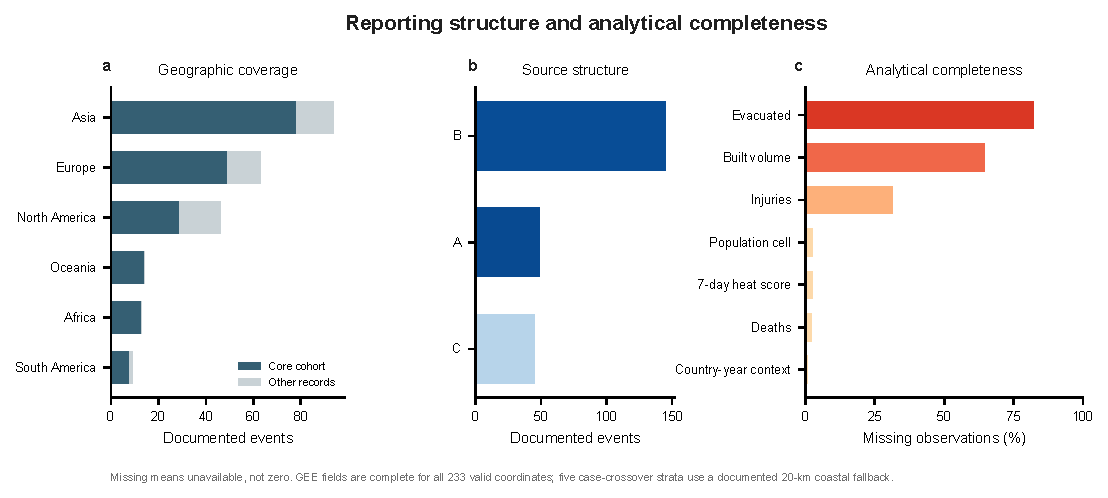
\includegraphics[width=\textwidth]{figures/Figure_S1.pdf}
\caption{\textbf{Reporting structure and analytical completeness.} \textbf{a}, Documented and core-cohort events by continent. \textbf{b}, Records by operational source grade; colour depth represents the core-cohort share. \textbf{c}, Missingness of reported consequence variables, country-year context and Earth Engine-linked variables after authenticated processing of all valid coordinates. Missing casualty values mean unavailable information and are not recoded as zero. Panel-level source data are exported by the figure notebook.}
\label{fig:s1}
\end{figure}

\begin{figure}[htbp]
\centering
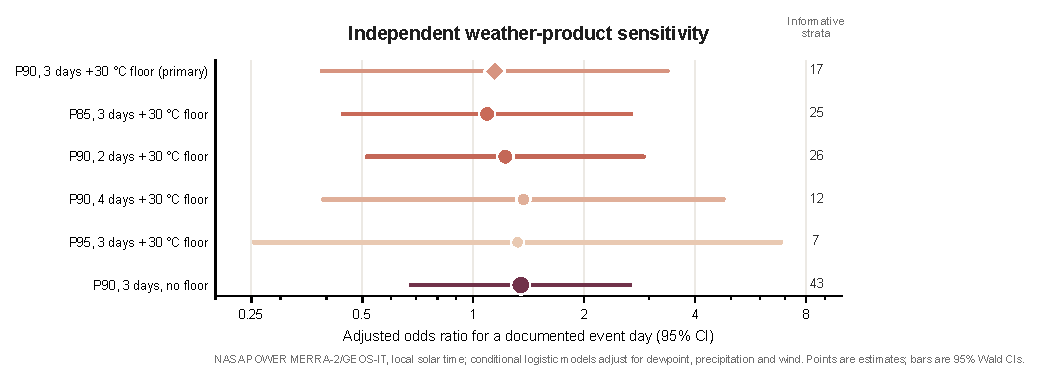
\includegraphics[width=\textwidth]{figures/Figure_S2.pdf}
\caption{\textbf{Independent weather-product sensitivity.} Adjusted odds ratios compare a heatwave-exposed with an unexposed documented event day in time-stratified conditional logistic models using NASA POWER MERRA-2/GEOS-IT meteorology. Points show estimates, horizontal bars show 95\% Wald confidence intervals, colour depth and point area encode the number of informative strata, and the diamond marks the prespecified primary definition. All models use 1,001 matched days in 228 strata and adjust for dewpoint, precipitation and wind; informative strata vary by heat definition as shown. Source data are provided in the panel-level source-data file.}
\label{fig:s2}
\end{figure}

\clearpage
\begin{figure}[htbp]
\centering
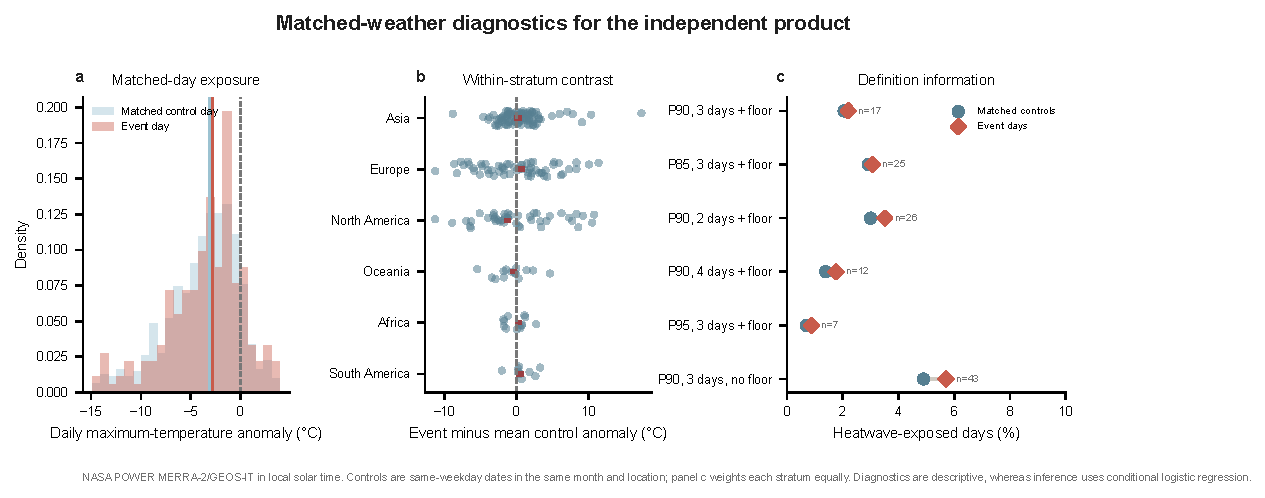
\includegraphics[width=\textwidth]{figures/Figure_S3.pdf}
\caption{\textbf{Matched-weather diagnostics for the independent product.} \textbf{a}, Density distributions of daily maximum-temperature anomalies on event days and matched control days; vertical lines mark group medians. \textbf{b}, Event-day anomaly minus the mean anomaly of matched control days in each stratum, grouped by continent; points are strata and red squares mark continent medians. \textbf{c}, Equal-stratum-weighted percentage of event days and matched control days classified as heatwave-exposed under the six prespecified definitions; labels give the number of informative strata. NASA POWER MERRA-2/GEOS-IT data use local solar time, and controls share the event location, calendar month, year and weekday. These panels diagnose exposure structure; inferential estimates come from the conditional logistic models in Supplementary Table~\ref{tab:s5}.}
\label{fig:s3}
\end{figure}

\clearpage
\begin{figure}[htbp]
\centering
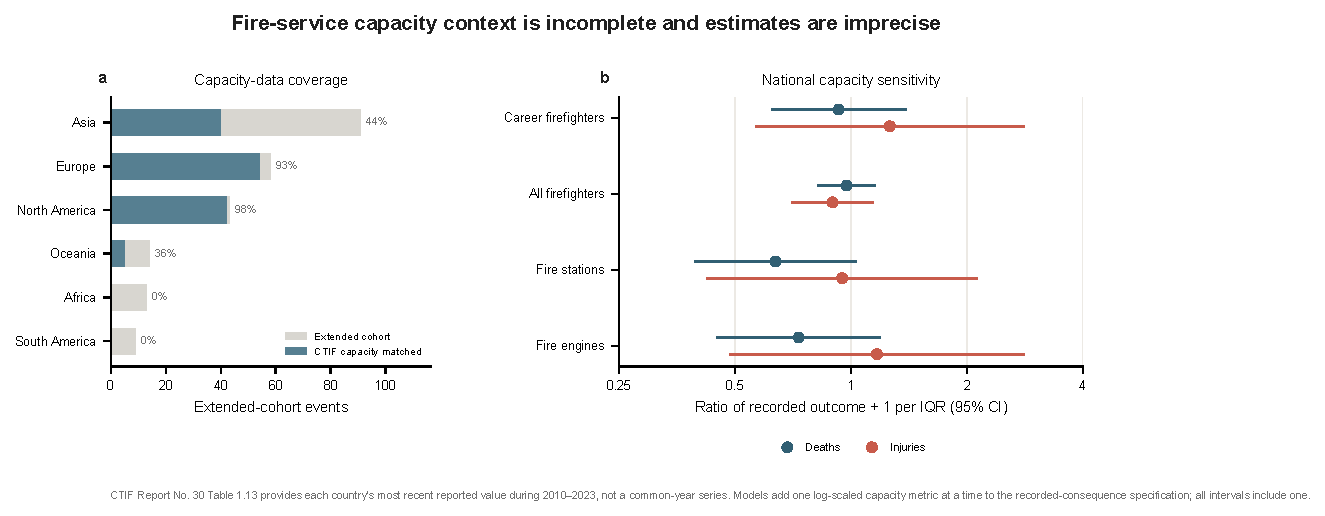
\includegraphics[width=\textwidth]{figures/Figure_S4.pdf}
\caption{\textbf{Coverage and sensitivity of national fire-service capacity data.} \textbf{a}, Extended-cohort event counts and the subset matched to a CTIF career-firefighter metric by continent; percentages denote event-level coverage. \textbf{b}, Exploratory adjusted ratios of recorded outcome plus one after adding one national capacity metric at a time. Points show estimates and horizontal bars show 95\% heteroskedasticity-consistent confidence intervals. CTIF Report No.~30 Table~1.13 supplies each country's most recent value during 2010--2023, not a common-year series. All intervals include one, and the estimates must not be interpreted causally or as evidence of no effect.}
\label{fig:s4}
\end{figure}

\clearpage
\begin{figure}[htbp]
\centering
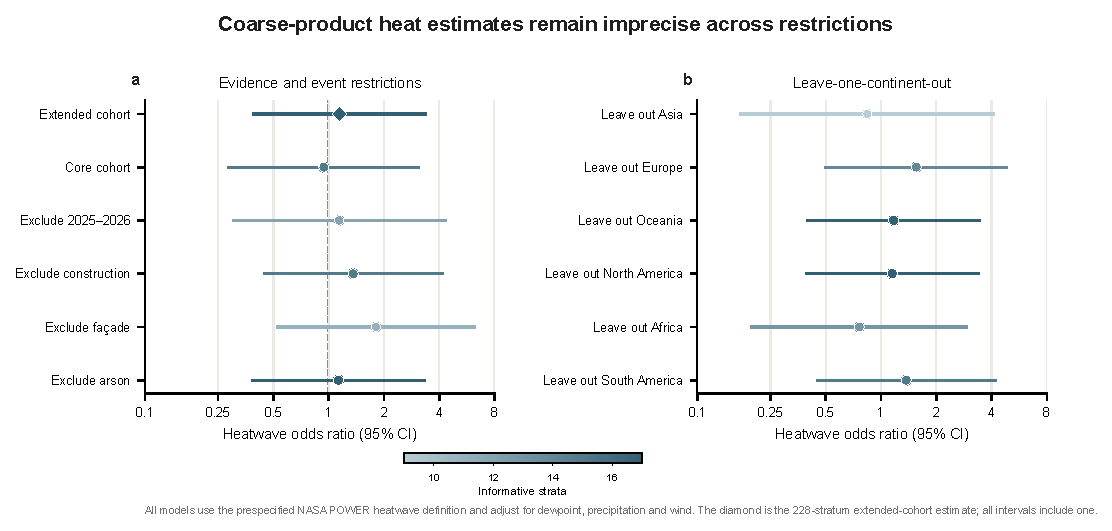
\includegraphics[width=\textwidth]{figures/Figure_S5.pdf}
\caption{\textbf{Evidence-window and geographic sensitivity of the independent weather product.} \textbf{a}, The NASA POWER primary heatwave definition in the extended and core cohorts and after prespecified period or event-type exclusions. \textbf{b}, The same model after leaving out each continent in turn. Points show adjusted odds ratios, horizontal bars show 95\% Wald confidence intervals, and colour and area encode the number of informative strata. The diamond marks the extended-cohort estimate. Every model adjusts for dewpoint, precipitation and wind; all intervals include one.}
\label{fig:s5}
\end{figure}

\clearpage
\begin{figure}[htbp]
\centering
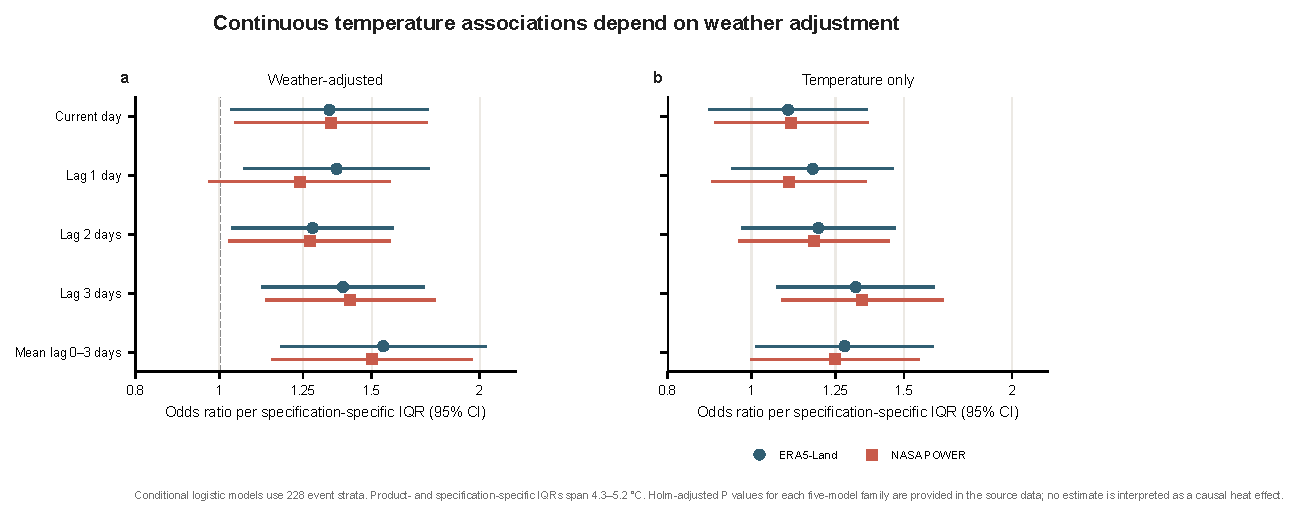
\includegraphics[width=\textwidth]{figures/Figure_S6.pdf}
\caption{\textbf{Continuous temperature associations depend on weather adjustment.} \textbf{a}, Conditional odds ratios per product- and specification-specific interquartile-range increase in maximum-temperature anomaly after simultaneous adjustment for dewpoint, precipitation and wind. \textbf{b}, Corresponding temperature-only estimates. Rows show the current day, lags one to three days and their four-day mean. Points distinguish ERA5-Land and NASA POWER; horizontal bars show 95\% Wald confidence intervals. All 228 strata are informative. Holm-adjusted $P$ values for each five-model product and adjustment family are reported in Supplementary Table~\ref{tab:s9} and the source data. These conditional associations are secondary and do not establish a heatwave or total-temperature effect.}
\label{fig:s6}
\end{figure}

\end{document}
